
\section{Security of third party apps}

\subsection{Permissions}
\subsection{App runtime}
\subsection{Simulator}
%\begin{figure}[h]
%    \centering
%    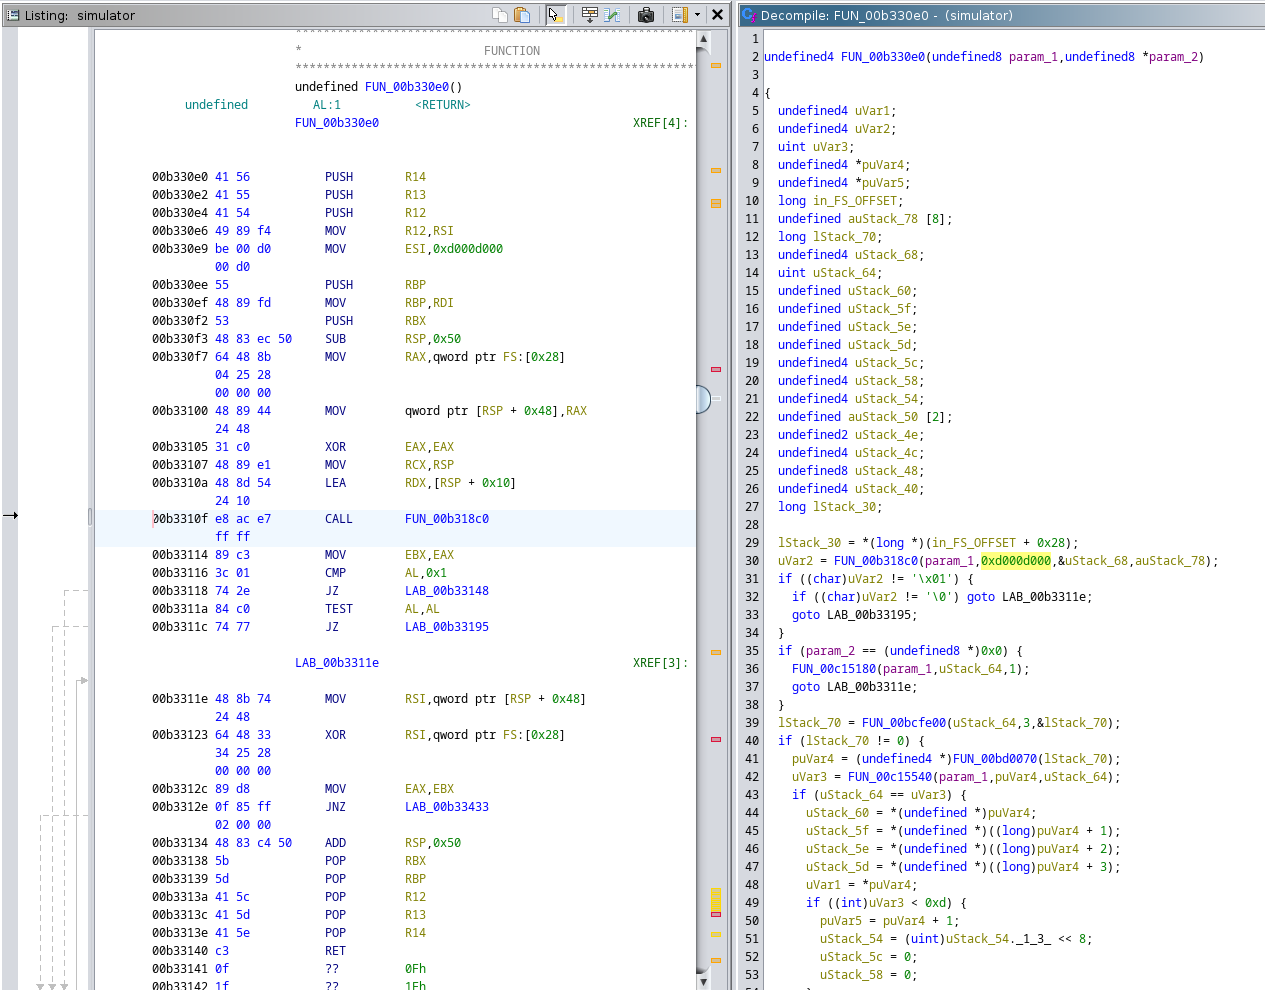
\includegraphics[width=1\linewidth]{images/ghidra.png}
%    \caption{Simulator decompilation}
%    \label{fig:concept}
%\end{figure}
Searching for value `0xD000D000` reveals two references in the code.
Based on the [article](https://www.atredis.com/blog/2020/11/4/garmin-forerunner-235-dion-blazakis) it is a PRG header tag.
The code doesn't look similar to the one included in the article.
Theoretically, I could try to analyze the logic for parsing the PRG file.
However, it doesn't seem like something that can be done in a reasonable amount of time.
\subsection{Building process}
The compiler is written in Java, which makes the analysis of the code relatively simple.
Nonetheless, the compilation is a complicated process consisting of several stages.
Java class `Opcode` contains a list of instructions in the final bytecode.
Additionally, SDK provides a mapping of all API methods to the number values, which is probably some type of address.

During the compilation, the code is translated to mid-level intermediate representation (MIR).
The files containing the representations are created during the build process and can be used for better understanding of the final artifact.
\subsection{Bytecode analysis}
\subsection{Modifying the executable}
In order to test the security of the virtual machine, it is useful to be able to edit the executable.
However, after changing the bytecode, it is necessary to sign the executable again.
After analysis of \textit{monkeybrains.jar} file, I created a kotlin script that signs the app again.
\subsection{Signing}
The generated app bytecode has to be signed by the developer.
The signing algorithm uses SHA1 hash of the bytecode that is signed with a private RSA key.
The key is 4096 long, which is more than recommended.

For the signing, conventions described in PKCS \#1 v2.2 are used.

SHA-1 is no longer considered secure against well-funded opponents.
NIST formally deprecated use of this hash function in 2011.
In 2020 there was a paper published demonstrating a chosen-prefix collision attack.
It still doesn't offer a viable solution to find a collision to a given hash for a chosen prefix.
However, the function has been already broken and in the upcoming years new attacks might be discovered.

Algorithm for signing:
- read bytes from PRG file that hasn't been signed yet
- don't include the bytes at the end of the file (called TERMINATOR in the code)
- compute the signature with Java security signature library (SHA1withRSA)
- Append the file bytes Developer signature, consisting of:
- magic number
- length of the whole signature
- signature
- modulus
- exponent
- Or in the case of the store signature:
- a different magic number
- length of the whole signature
- signature
- Append the terminating bytes that were skipped before

\subsection{Communication between the watch and the phone}

\subsubsection{Garmin communication between the Android apps}
Garmin apps define their own permissions.
One of them is for example \verb|com.garmin.android.apps.connectmobile.permission.RECEIVE_BROADCASTS|, which allows to listen for action \verb|ACTION_ON_FIND_MY_PHONE_MESSAGE_RECEIVED|, which triggers sound on the phone.
I don't know, however, who sends this action.

\textbf{Privacy issue 1} - Every app can register for garmin ConnectIQ service without registering any permissions.
It can give the information if and what Garmin device the user has connected to the phone.

It seems like any phone app can receive events from all watch apps.
There is no authentication.

I have a proof of concept, but idk which apps are using it, if any\ldots

According to Android documentation: [About broadcasts](https://developer.android.com/guide/components/broadcasts),
it is possible to send broadcasts that can be only received by apps with specific permissions.
It is also possible to define a custom permission.
However, custom permissions have to be already defined when such app is being installed.
Because of that, it is probably not a viable option for Garmin.

%\begin{figure}[h]
%    \centering
%    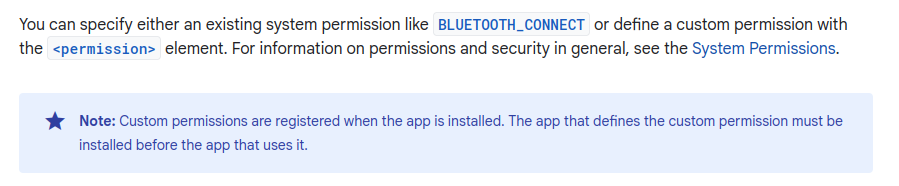
\includegraphics[width=1\linewidth]{images/android-custom-permissions-note.png}
%    \caption{Android custom permissions note}
%    \label{fig:concept}
%\end{figure}

\textbf{Privacy issue 2} - Third party apps can user's personal information or access the internet.
To do so, they need to request permission, specific to the used module.
For example, `Communications`, `Fit`, `Positioning`.
This system offers some granularity, and the user can see what data will the app have access to.
However, in February 2023, Garmin introduced a new module: Complications.
It is a publish/subscribe model that allows for the apps to publish different metrics, so that they would be accessible for any watch face.
However, it should be considered that it removes the granularity of permissions.
Every app can potentially publish very sensitive data.
And every watch face can access all this data if it requests `Complications` permission.

\subsection{Sandboxing}
\subsection{App sideloading}